%
% This file works for Adobe Distiller as the PDF creator, with drivers dvips or dvipsone.
% It also works for pdftex (and luatex), dvipdfm, dvipdfmx, and xetex.
%
\documentclass[11pt]{article}
\usepackage{amsmath}
\usepackage[forcolorpaper,pro]{web}
\usepackage{eforms}
\usepackage[!preview,!viewMagWin]{fitr}
\usepackage[js=restoreHookBlink,js=jmpHookBlink]{lmacs}
\usepackage{graphicx}

\DeclareDocInfo
{%
    title={Jumping to a Rectangular Region},
    author={D. P. Story},
    university=My University,
    talkdate={Dec.\ 17, \the\year},
    subject={Demo file to test the FitR view destination of PDF},
    keywords={LaTeX, PDF, Acrobat, JavaScript},
    university={%
            Acro\!\TeX.Net\\
        NORTHWEST FLORIDA STATE COLLEGE\\
           Department of Mathematics},
    email={dpstory@acrotex.net},
    version={1.0},
    copyrightyears={2012}
}
\nocopyright
\norevisionLabel

\selectColors{linkColor=blue}

\parindent0pt \parskip6pt \pagestyle{empty}

% \renewcommand{\overlayPresets}{\H{I}\S{D}\BG{}\BC{blue}}
% \renewcommand{\allowFXDefault}{false}

\begin{document}
\begin{center}\sffamily\bfseries\Large\color{blue}
    Jumping to a Rectangular Region\\[1ex]\normalsize\normalcolor
    Dr. D. P. Story, \href{http://www.acrotex.net}{Acro\!\TeX.NeT}
\end{center}

\textbf{Introduction.} This document demonstrates a technique designed to
help people with low vision read material by providing them with a
convenient way to magnify specific regions of the document. This is
especially useful for reading technical material such as mathematics, as
is demonstrated here.

\textbf{Instructions:} Click on any of the mathematics to magnify a region
around it, the border will blink briefly to focus your attention on it.
To restore the previous view, click on the region again,
the formula is briefly highlighted by a blinking border so
can quickly find your place in the document.


\textbf{Sample Mathematical Text.} Consider the problem of numerically
solving the first order differential equation
\jdRect*[adddestw=60,adddesth=20]{$y'=f(t,y)$} on
\jdRect*[adddestw=1in,adddesth=30]{$[t_{start}, t_{end}]$}. Suppose we
want to classify third order \textsf{Runge-Kutta} type methods. Start with
\begin{align*}
\jdRect[height=1.3in,width=2.6in,lift=16pt,shift=-15pt,adddestw=10,adddesth=10] %
K_1 &= hf(t_n, y_n)\\
K_2 &= hf(t_n +r h, y_n+aK_1)\\
K_3 &= hf(t_n +s h, y_n+bK_1+cK_2)\\
K &= w_1 K_1+ w_2 K_2+ w_3 K_3\\
y_{n+1} &= y_n+K
\end{align*}
Find the system of equations satisfied by
\jdRect*[adddestw=10,adddesth=10]{$r,s, a, b, c, w_1, w_2, w_3$}
that will make the above algorithm a third order method.

\textbf{Inline links.} Links can be provided within the text to jump to a
magnified region that needs to be inspected more closely. The links below
are different from the ones above. After jumping to a magnified rectangle,
restore the preview view by clicking on the rectangle.

\def\RungePic{\includegraphics[width=\marginparwidth]{runge}}
\def\KuttaPic{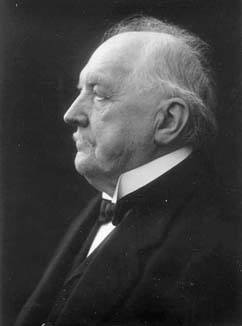
\includegraphics[width=\marginparwidth]{Kutta}}
\def\jrOpts#1#2{link=#1,dest=#2}

\textbf{\jdRect*[nodest,\jrOpts{jmp}{rungePic},adddestw=10,adddesth=10]{Carl Runge}}%
\marginpar{\jdRect*[\jrOpts{restore}{rungePic},adddestw=\marginparsep,
adddesth=\marginparpush]{\parbox[b]{\marginparwidth}{\RungePic\\
\normalcolor\centering\footnotesize\textsf{Carl Runge}}}} (1867-1944)
was the third of four sons from a well-to-do German merchant family.  He
is remembered for his \textsf{Runge-Kutta} method for solving
differential equations.

\textbf{\jdRect*[nodest,\jrOpts{jmp}{KuttaPic}]{Martin Kutta}}%
\marginpar{\jdRect*[\jrOpts{restore}{KuttaPic},adddestw=\marginparsep,
adddesth=\marginparpush]{\parbox[b]{\marginparwidth}{\KuttaPic\\
\normalcolor\centering\footnotesize\textsf{Martin Kutta}}}} (1867-1944)
extended the Runge's method of solving ordinary differential equations. He
is also known for his work on airfoils.

% Again, don't forget to press
%\textbf{Alt+Left Arrow} to return to the view you had before you clicked
%on the link.

\begin{flushright}
This work was  motivated by Mohsen M.
\end{flushright}
\end{document}
